\section{Benchmark NIST-2 "Reentrant Corner"}
\label{sec:bench-2}

This is a standard benchmark for adaptive FEM algorithms.
A reentrant corner is nothing more than an internal or inside corner.
The problem of reentrant corner happens very often, 
because of the reentrant corner, the error estimate 
of the domain does not get convergece or get slow convergence.
The exact solution of this problem is smooth but contains 
singular gradient in the reentrant corner.
The equation solved is the Laplace's equation.

\begin{equation} \label{laplace}
-\Delta u = 0,
\end{equation}
in the domain $\Omega = (-1, 1)^2$, with a unit square section
removed from the bottom part of positive $x$ axis.
Equation (\ref{laplace}) equipped with Dirichlet
boundary conditions given by the exact solution:

\begin{equation}\label{exact-nist-2}
u(x, y) = r^{\alpha}\sin(\alpha \theta),
\end{equation}
where $\alpha = \pi / \omega$, $r = \sqrt{x^2+y^2}$, and $\theta = tan^{-1}(y/x)$. Here $\omega $ determines
the angle of the reentrant corner.
The solution of NIST-2 with $\omega = 3 \pi / 2$  is shown in Fig. \ref{fig:sln-nist02}.

\begin{figure}[!ht]
\centering
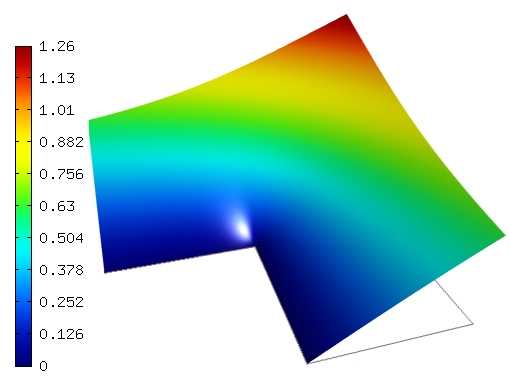
\includegraphics[height=6cm]{nist/nist-2/solution.png}
\caption{The solution to NIST-2 benchmark problem.}
\label{fig:sln-nist02}
\end{figure}
